\icode{N24-MD-CA-L3-261112-004}
\nceeID[14]{2024新课标}{12}
如图，一长度\(l =\) \,\qty{1.0}{m}的均匀薄板初始时静止在一光滑平台上，薄板的右端与平台的边缘\(O\)对齐。薄板上的一小物块从薄板的左端以某一初速度向右滑动，当薄板运动的距离\(\Delta l = \frac{1}{6}l\)一时，物块从薄板右端水平飞出；当物块落到地面时，薄板中心恰好运动到\(O\)点。已知物块与薄板的质量相，它们之间的动摩擦因数\(\mu = 0.3\)，重力加速度大小\(g =\)\,\qty{10}{m/s^2}。求
\begin{enumerate}
	\item 物块初速度大小及其在薄板上运动的时间；
	\item 平台距地面的高度。
\end{enumerate}

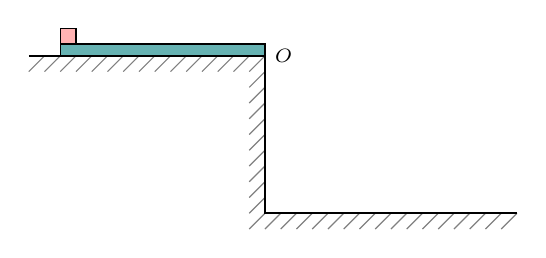
\begin{tikzpicture}[font=\scriptsize]
	\foreach \x in {-3,-2.8,...,-.4}
		\draw[gray] (\x,-.2)--++(.2,.2);
	\foreach \x in {0,.2,...,3}
		\draw[gray] (\x,-2.2)--++(.2,.2);
	\foreach \y in {-.2,-.4,...,-2.2}
		\draw[gray] (-.2,\y)--++(.2,.2);
	\draw[thick] (-3,0)--(0,0)--(0,-2)--(3.2,-2);
	\draw[fill=teal!60] (-2.6,0) rectangle(0,.15);
	\draw[fill=red!30] (-2.6,.15) rectangle(-2.4,.35);
	\node at(0,0)[right]{\(O\)};
\end{tikzpicture}
\begin{answer}
    
\end{answer}